\section{Controlled experiment and data}
\label{S:data}
\subsection{VIRE}
Virtual Immersive Reality Experiment (VIRE) is used in this study as the tool to develop the controlled experiments and collect the required data. We selected virtual reality, as our experiments involve situations that are either dangerous in reality and may result in disastrous outcomes, or are futuristic scenarios that are not yet feasible to implement. On the other hand, stated preferences surveys, which are the conventional tool of data collection in similar studies, cannot provide naturalistic datasets as participants have no prior exposure to automated vehicles.

 VIRE is an in-house developed virtual reality framework designed for experiments in controlled environments~\citep{farooq2018virtual}. The unique feature of VIRE is that the virtual objects are designed such that they react to the participant's actions. For instance, if a participant is crossing the road, based on their location, the approaching vehicle may slow down or completely stop, thus giving a dynamic, immersive, and realistic experience. A scenario is generated based on a set of variables and then it is projected onto the eyes of participants through an immersive head mounted display. Participants, finding themselves on a simulated 3D sidewalk, are asked to start crossing when they feel it is comfortable to do so. During the experiments, data on the movements of pedestrians are recorded using motion sensors and the reactions of virtual objects are computed in real-time.

Each scenario is defined by 9 controlled variables, which are selected based on related literature on future urban streets~\citep{kinaSUR}, while considering the available facilities. These variables are categorized as follows: 
\begin{itemize} 
\item \textbf{Rules and regulations:} speed limit, minimum allowed gap time between vehicles 
\item \textbf{Street design:} lane width, type of road 
\item \textbf{Automated vehicles:} traffic automation status, number of braking levels
\item \textbf{Demand:} traffic flow (arrival rate)
\item \textbf{Environmental conditions:} time of day, weather.
\end{itemize}
Multiple levels are defined for each of the controlled variables, as presented in \cref{tab:levels}. The standards of speed limit, suggested minimum gap between cars and lane width at the time of experiment in a typical road in downtown Toronto were 50 \textit{km/hr}, 2 \textit{sec}, and 3 \textit{m}, respectively. To take into account future possible modifications to the current standards, one of the levels for each of these three variables are set in our experiment to have the same value of a typical Toronto street standard, with the other two levels considering possible changes. Number of braking levels, which is only defined for automated vehicles, represents the level of smoothness of braking system of the AVs. Having a greater number of levels shows a more smooth deceleration when AVs face a barrier. Level 1 system for braking means the vehicle decelerated with a constant rate as long as a barrier (crossing pedestrian in our case) is observed on the road. In level 2 systems for braking, the AV first decelerates to a speed equal to the half of its initial speed in half of their initial distance to the barrier. If the barrier still exists, the AV will change the deceleration to fully stop for the barrier in the rest of the distance. Similar pattern exists for level 3 braking system with three deceleration rates calculated and applied. On the other hand, braking for all human-driven vehicles are defined as level 1. Details on how the braking levels work, as well as sample velocity profiles of a hypothetical vehicle under different braking levels are provided in \cref{A:brake}. Simulated traffic on the road can either be fully human-driven, fully automated or a mixture of automated vehicles and human-driven cars. In the experiments, users distinguish human-driven and automated vehicles by observing the absence of a driver in the driving seat in AVs, and a box-shaped LiDAR sensor on top of them. Similar to \citep{jayaraman2019pedestrian}, participants get familiar with the shape of AVs in the training before the experiments, so that they can tell the difference between the two types of vehicles. Moreover, AVs and human-driven cars are different in braking systems, which might not be realized by the participants, unless they do the experiment as such that a vehicle has to brake for them. As for the demand on the road, values are extracted from flow rates on a typical road in downtown Toronto during off hour and peak hour hourly average (530 and 1100 \textit{veh/hr/lane} respectively) and the mean value of these flow rates (750 \textit{veh/hr/lane}). Two flow variables are also derived based on the controlled variables and used in the analysis: distance between cars and traffic density. Finally, the environmental conditions in the simulation are designed as such that participants experience day and night time of the day, as well as clear and snowy weather, in which the sight distance of pedestrians is affected. All the collected variables using VR, as well as those collected through the questionnaires before the experiments are described in \cref{A:var} While doing the experiments, coordinates and head orientations of participants are recorded in intervals of 100 milliseconds, as well as the coordinates of simulated vehicles. 

\begin{table}[!h]
\caption{Controlled variables and their levels}
\setlength\extrarowheight{2pt}
\centering
\scalebox{0.7}{
\begin{tabular}{|l|l|*{30}{p{\lena}|}}
\hline
\textbf{Factor}&\textbf{Variable}           & \multicolumn{30}{c|}{\textbf{Levels}}\\
\hline\hline  
\multirow{2}{*}{\textbf{\begin{tabular}[c]{@{}l@{}}Rules and\\ regulations\end{tabular}}}&Speed limit (km/h) & \mcii{30} & \mcii{40} & \mcii{50} \\
\cline{2-5}
&Minimum allowed gap time (s) & \mcii{1} & \mcii{1.5} & \mcii{2} \\  
\hline
\multirow{2}{*}{\textbf{Street design}}&Lane width (m) & \mcii{2.5} & \mcii{2.75} & \mcii{3} \\  
\cline{2-5}
&Road type & \mcii{1-way} & \mcii{2-way} & \mcii{2-way with median} \\  
\hline
\multirow{2}{*}{\textbf{\begin{tabular}[c]{@{}l@{}}Automated\\ vehicles\end{tabular}}} &No. of braking levels &  \mcii{1} & \mcii{2} & \mcii{3} \\  
\cline{2-5}
&Traffic automation status& \mcii{Fully human-driven} & \mcii{Mixed traffic} & \mcii{Fully automated} \\  
\hline
\textbf{Demand}&Arrival rate (veh/hr) & \mcii{530} & \mcii{750} & \mcii{1100} \\  
\hline
\multirow{2}{*}{\textbf{Environmental}}&Time of day & \mciii{Day} & \mciii{Night}  \\
\cline{2-5}&Weather & \mciii{Clear} & \mciii{Snowy}  \\
\hline
\end{tabular}}
\label{tab:levels}
\end{table}

Scenarios are then generated based on the above-mentioned controlled variables. Each possible combination of different levels of controlled variables is a potential scenario. To select the scenarios for the experiments, a design of experiment is conducted, which is described in detail in the next section. 

\subsection{Design of experiment}
To study the effects of various different attributes on pedestrians' crossing behaviour, a design of experiment (DoE) needs to be conducted. The first and simplest method for DoE is full factorial design, in which after assigning different levels to each attribute, all possible combinations of different attributes' levels are considered for the experiment. In our case, however, this is an impossible approach to take as there would be a total of 8,747 possible combinations based on the 9 attributes we defined and their levels. To overcome this problem, several \textit{Fractional Factorial Designs} have been developed based on the objectives of the design, models to be developed and the amount of prior information available~\citep{cavalcante2011bayesian}. In fractional factorial designs, a subset of choice tasks are selected. The most widely used strategy for selecting a subset of tasks is orthogonal design, in which tasks are selected in a way to produce zero correlation between attributes~\citep{ortuzar1994modelling}. However, orthogonality may limit the experiment design by putting constraints in terms of the number of runs required and possible settings for factor levels. Recent studies on the topic have led to \textit{Optimal Designs}, which focus on the efficiency of the experiment, rather than orthogonality~\citep{rose2009constructing}. In optimal and efficient designs researchers try to find the efficient design in terms of a selected measure of quality for parameters' estimates. In the most widely used optimal design, D-Optimal design, for instance, variances and covariances of parameter estimates determine attribute level combinations~\citep{atkinson2007optimum}. For the purpose of data collection for this study, we use an optimal design of experiment, as it allows experiments to be conducted in a more flexible manner in terms of number of runs required and tasks to be observed. 

In D-Optimal designs, a number of assumptions and parameter estimates for the model are required in order to calculate covariance matrix, as this matrix varies based on the model used. In order to deal with parameter priors required in these methods, two approaches can be taken. First approach is to consider parameter priors to be zero, which is called the null hypothesis~\citep{street2005quick}. This assumption indirectly results in the orthogonality of null hypothesis D-Optimal designs. In addition, it is assumed in this type of methods that the model used is Multinomial Logit (MNL). Not requiring a priori knowledge on parameter estimates makes this method useful when no prior information is available. The second approach, on the other hand, assumes that some estimates are available on the values of parameters. Rose and Bliemer suggested that a priori parameter estimates can be obtained from: the literature, pilot studies, focus groups and expert judgments~\citep{rose2008designing}. The main advantage of this approach is that it enable researchers to use any model type, in contrary to the former approach that was applicable only to MNL.

In this study, we obtained estimates on a priori parameters based on a trial experiment on a limited number of participants. To do so, a demo of the data collection was conducted with 5 participants, each going through 30 randomly selected scenarios to get an initial idea on the model parameters. As the objective of the data collection was to obtain required data to model pedestrian wait time, we assumed a cox proportional hazards model (CPH) for waiting time. Thus, a design of experiment was developed based on the CPH model on the trial data, and top scenarios based on importance weights were selected for our experiment. In total, 90 different scenarios were selected. The design of experiment formulation for wait time modelling, which is the topic of interest in this study is presented in~\cref{A:design}.

\subsection{Data collection campaign}
Data collection campaign for this study started in April 2018, as a trial experiment with a limited number of participants, and then continued with main experiments until September 2018. In total, 180 people participated in the experiments, 160 of which succeeded to complete at least one of their tasks in the experiment. These 160 participants consisted of 113 adults, and 47 kids and teenagers. To make the data as inclusive and heterogeneous as possible, we conducted our experiment in four different locations. Started at Ryerson University with post-secondary students, we then moved to Toronto City Hall and North York Civic Center to include professionals in the field who were more familiar with the nature of the experiments and the questions we were trying to answer. We repeated the experiments in Markham City Library, in which we included general public. Finally, we had our experiments with Maxim City summer school, which included kids and teenagers between 9 to 15 years old. In \cref{fig:vire}, a view of a sample scenario and the experiment setup with participants is shown. A video of a participant, while doing the experiment is also attached in the supplementary materials.

\begin{figure}[!ht]
\begin{adjustbox}{varwidth=\textwidth,fbox,center}
\centering
\begin{subfigure}{0.8\linewidth}

    \begin{subfigure}[b]{0.5\textwidth}
         \centering
         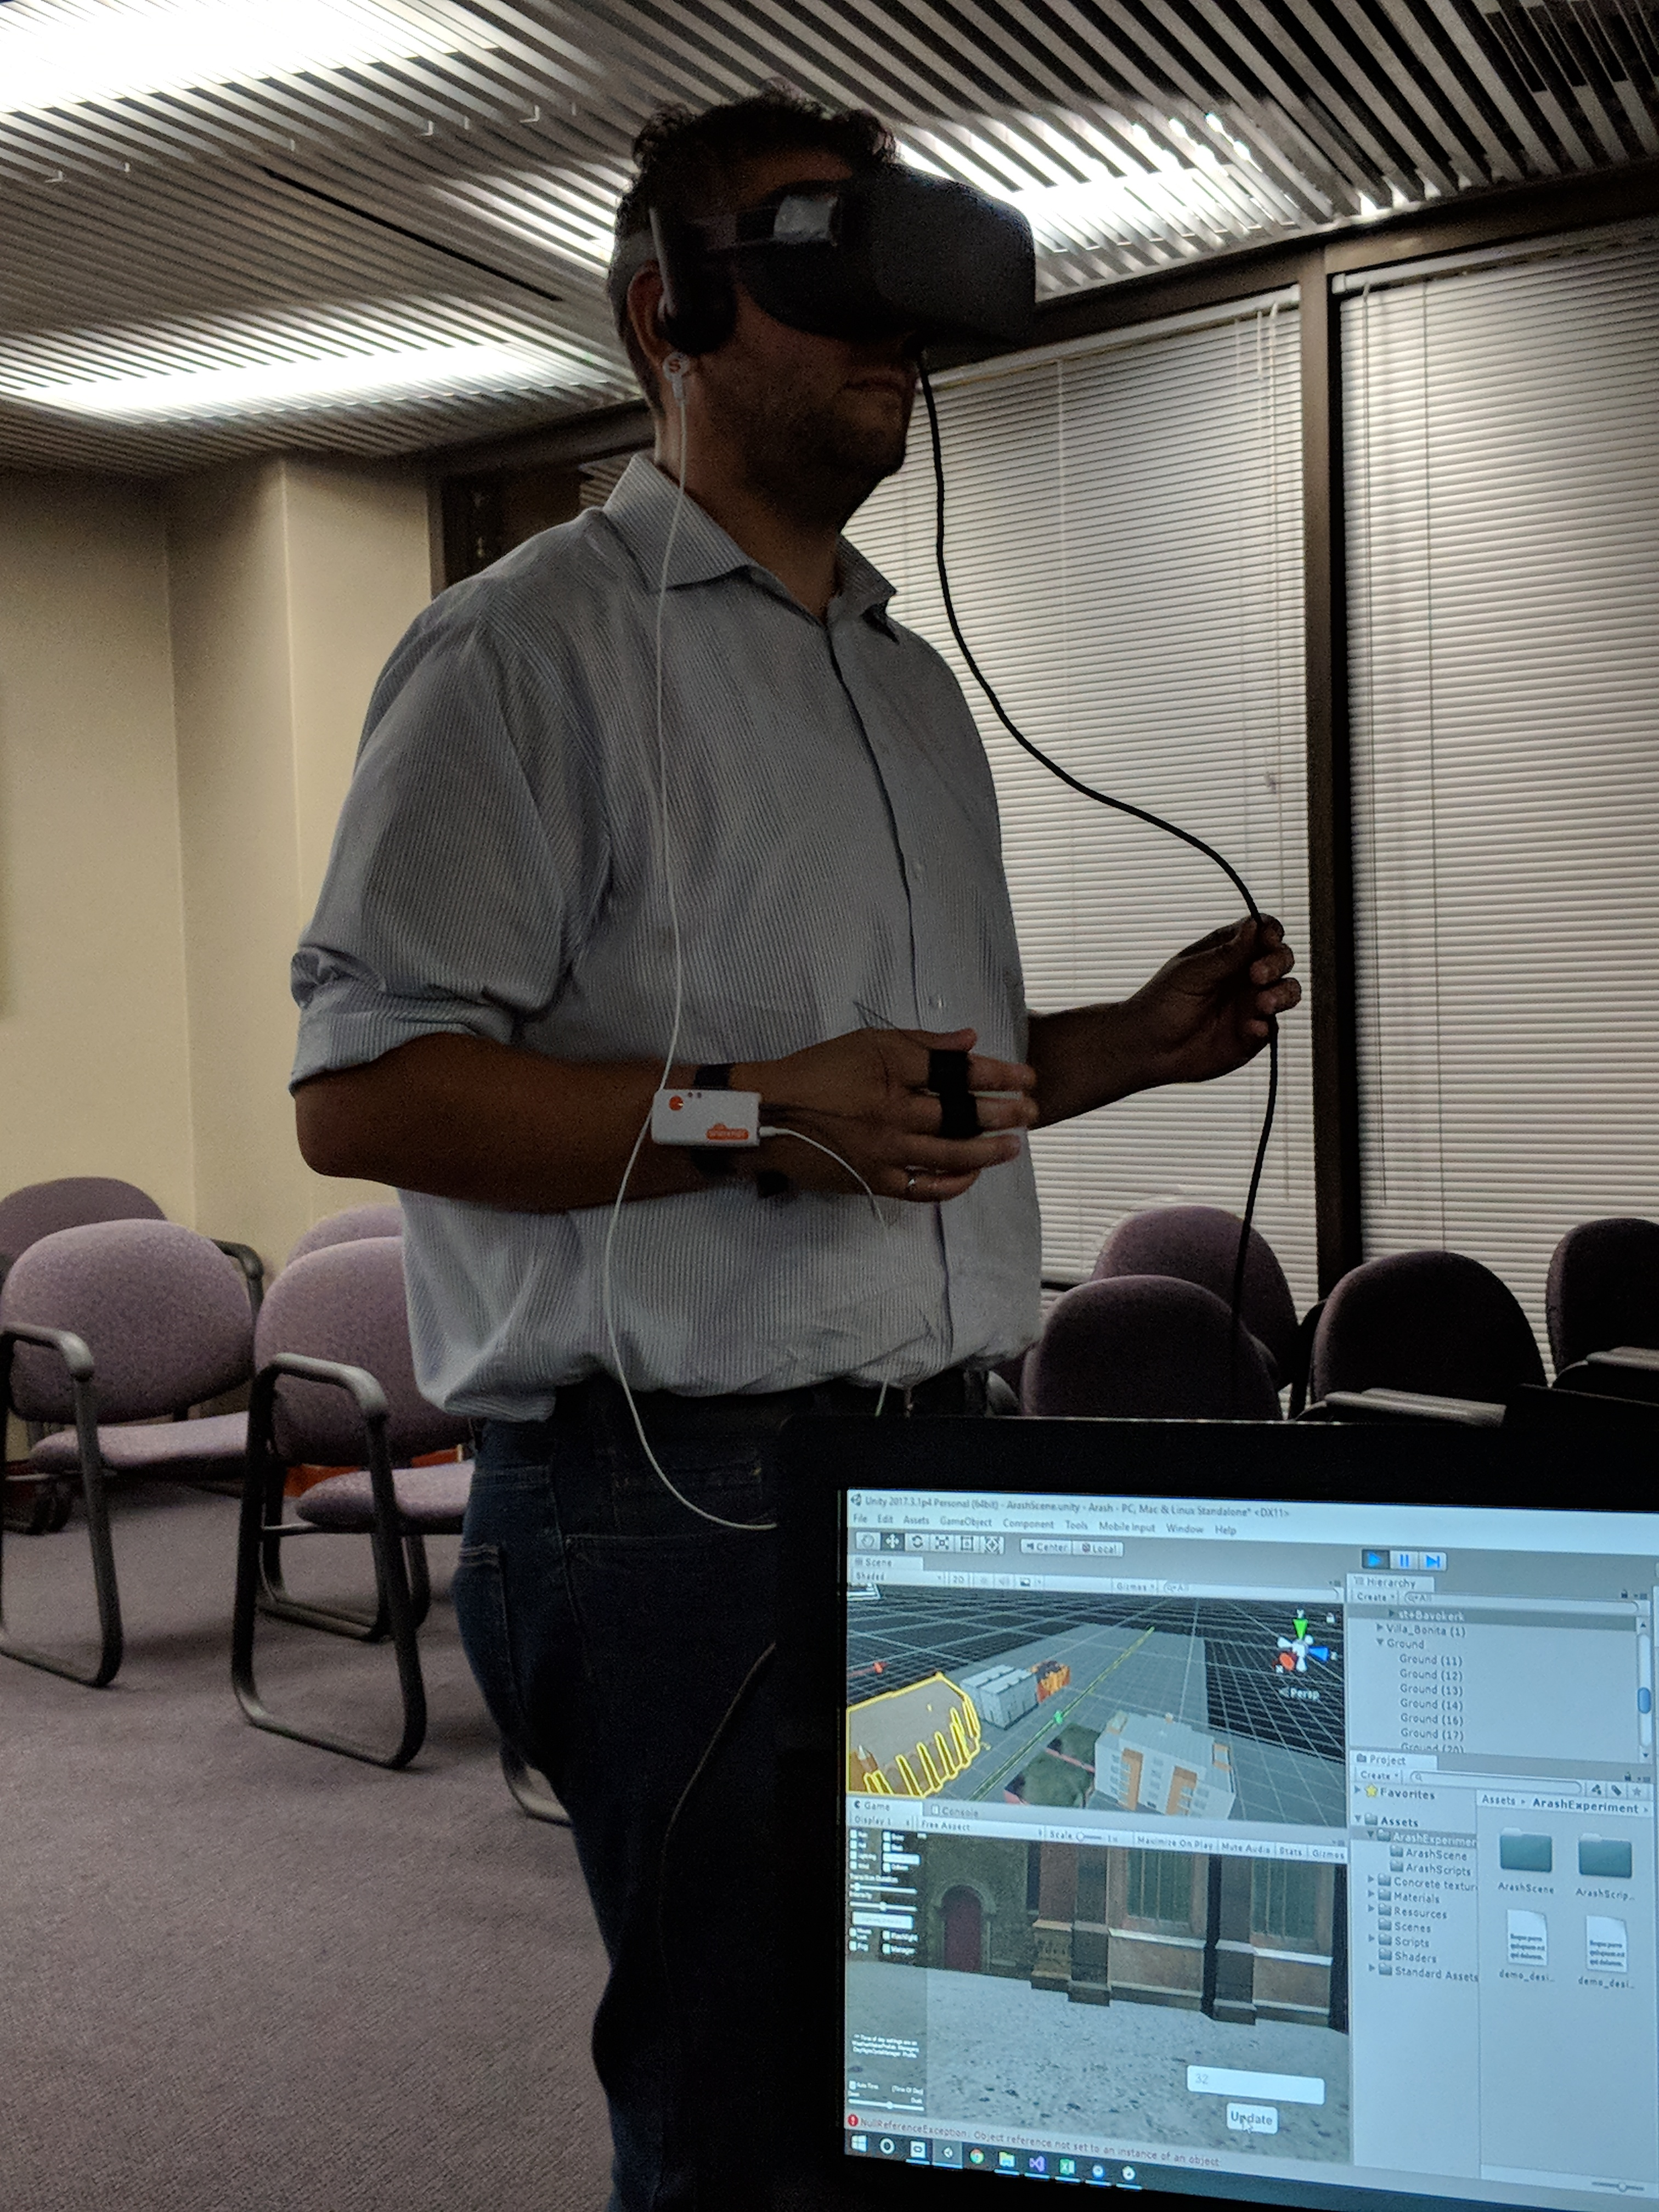
\includegraphics[trim=100 100 100 175,clip,
         scale=0.06]{chapter_4/figures/participant.jpg}
         \caption{A participant in Toronto City Hall}
     \end{subfigure}
     \hfill
     \begin{subfigure}[b]{0.5\textwidth}
         \centering
         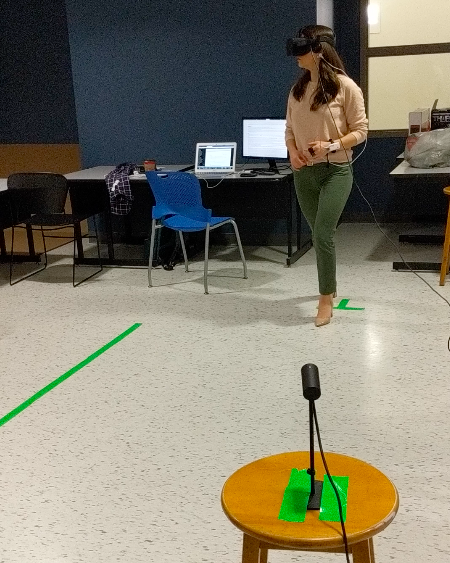
\includegraphics[scale=0.4]{chapter_4/figures/img1.png}
         \caption{A participant at Ryerson University}
     \end{subfigure}
\end{subfigure}\\[2ex]
\begin{subfigure}{0.8\linewidth}

\centering
\includegraphics[scale=0.1]{chapter_4/figures/vr1.png}
\caption{A virtual sample environment}
\end{subfigure}
\end{adjustbox}

\caption{A sample view of experiments}
\label{fig:vire}
\end{figure}

The process of an experiment for a participant is as follows: The participant is first asked to fill a questionnaire on his/her sociodemographic information, travel patterns and previous experiences with virtual reality (See \cref{A:var} for details of information collected). The participant is then familiarized with the VR environment for 5 minutes. After familiarization, 15 scenarios are randomly drawn from the 90 selected scenarios by the experiment design. After a scenario starts, the participant finds him or herself on the sidewalk of a marked crossroad, with vehicles approaching. The participant then have to decide to initiate his or her cross when he or she feels it is safe to do so. If a pedestrian starts crossing the street, approaching vehicles will detect them and apply braking depending on the scenario to slow down and avoid a collision. The vehicles will continued to move after the street is cleared. In this study, we solely investigate safe crosses of pedestrians. Thus, dangerous crossings with a Post Encroachment Time (PET) of less than 1.5 seconds are removed from the data and not considered in this study. For an adult participant, each scenario is conducted two times, accumulating to 30 total experiments with a total time of about 30 minutes. Our trial study showed that continuing experiments for over 30 minutes causes fatigue among participants and thus the results may be affected. For adolescent participants, each scenario is conducted once, with a total time of 15 minutes for the whole experiment. It should be noted that data from child participants are not used in this particular study as their behaviour when facing VR environment and AVs mostly involved unpredicted reactions and crossing behaviour, and we believe a different data cleaning is required on their data. A video of a young participant, while doing the experiment is provided in the supplementary materials.
\subsection{Data summary}
Before applying feature selection algorithms, the first step in data preprocessing would be to remove highly correlated variables from the dataset. To do so, Variable Inflation Factor of covariates are calculated, which for each covariate represent the multicollinearity of that covariate. In general, a higher VIF for a covariate indicates the higher ability to predict that covariate using linear regression based on other covariates on the dataset. After removing experiments where pedestrians could not complete the crossing, or could not follow the experiments' procedures, a total of 2,291 responses were remained to be studied. Collected data are then used to estimate models for predicting pedestrian waiting time. In \cref{fig:waitfreq}, the frequencies of crosses with different wait times are provided. As it can be inferred from this figure, a majority of the crosses (54\%) occurred in the first two seconds, decaying exponentially. According to the figure, Only 6\% of the crossings took more than 20 seconds of wait time.
\begin{figure}[]
    \centering
    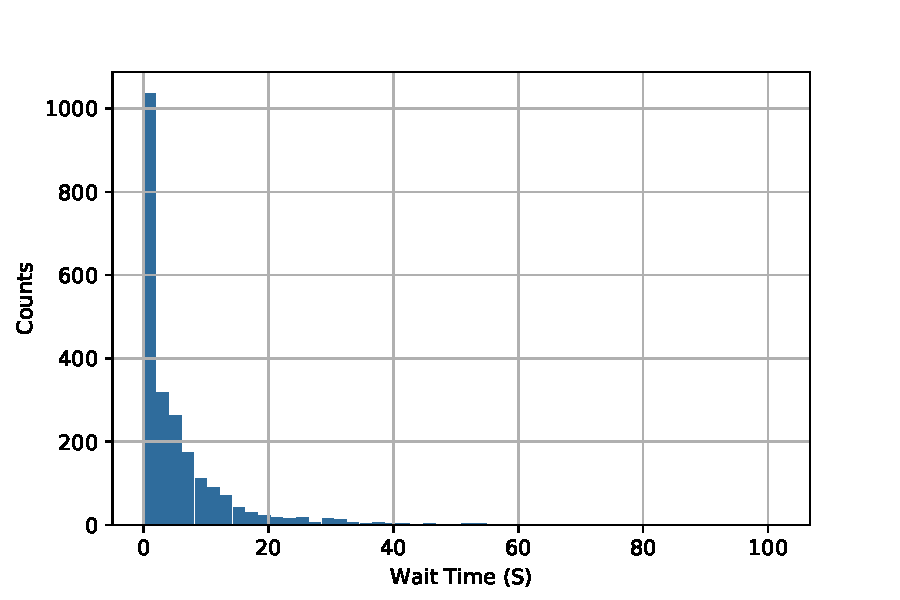
\includegraphics[scale=0.6]{chapter_4/figures/waitfreq.pdf}
    \caption{Wait time frequency}
    \label{fig:waitfreq}
\end{figure}
All quartiles of waiting time for participants, as well as the average waiting time, are depicted thorough box plots in \cref{fig:comparison} for different levels of all covariates. As shown in the figure, more participants in our experiment tended to wait longer when exposed to automated vehicles, and in mixed traffic conditions participants even took longer to cross, compared to fully automated conditions. The reason might be the effect of having two different types of vehicles in these scenarios, which increases uncertainty among participants. In the second plot, waiting time over different levels of speed limit, is not as expected. Participants in our sample data waited longer in slower traffics. The reason for this behaviour can be that participants waited for a number of vehicles in scene to pass first before crossing, which takes longer for slow vehicles. Moreover, given a fixed arrival rate, higher speeds mean larger gap distances between the vehicles, which makes it easier for pedestrians to cross. Considering pedestrians tendency to decide to cross based on their distance to the vehicles, other traffic parameters like density and flow are also analyzed to complement speed limit. The next box plot reveals that in wider lane widths, participants in our experiment waited longer before crossing. No observable difference is identified in the median of minimum gap time allowed, with 1 second gap times having a slightly higher wait times compared to 2 seconds gap times. According to the arrival rate box plot, participants in more congested areas with higher traffic flows waited longer before crossing. Higher values for derived variable of vehicles' density also had a positive correlation with waiting time. Values of density are continuous in the experiment, and are categorized to three equal intervals in the figure. Three defined braking types for automated vehicles are shown next. As participants are not informed about the type of braking level before the experiments, it seems that a particular trend does not exist with them and waiting time. Two-way roads with median seemed to result in shorter waiting times compared to two-way roads with no median. Regarding environmental variables, no notable pattern based on weather conditions and time of the day is seen in the plots. 
In the age categories analyzed, two extremes of the analyzed age groups have greater waiting time, and in gender, females have slightly longer wait times.
Five next plots are relevant to travel habits of participants. Almost all of these plots show longer wait times for participants who tend to have less tendency to have active modes of transportation. Finally, participants who have prior experience in using virtual reality wait shorter on the sidewalk, as they probably feel more comfortable using the devices. Average, standard deviation and p-values for comparison on means of all the covariates depicted in box plots of \cref{fig:comparison} are presented in \cref{A:data}. It should be noted that a detailed analysis of covariates require developing survival models, which are presented in detail in \cref{S:results}. 

\begin{figure}[H]
    \centering
    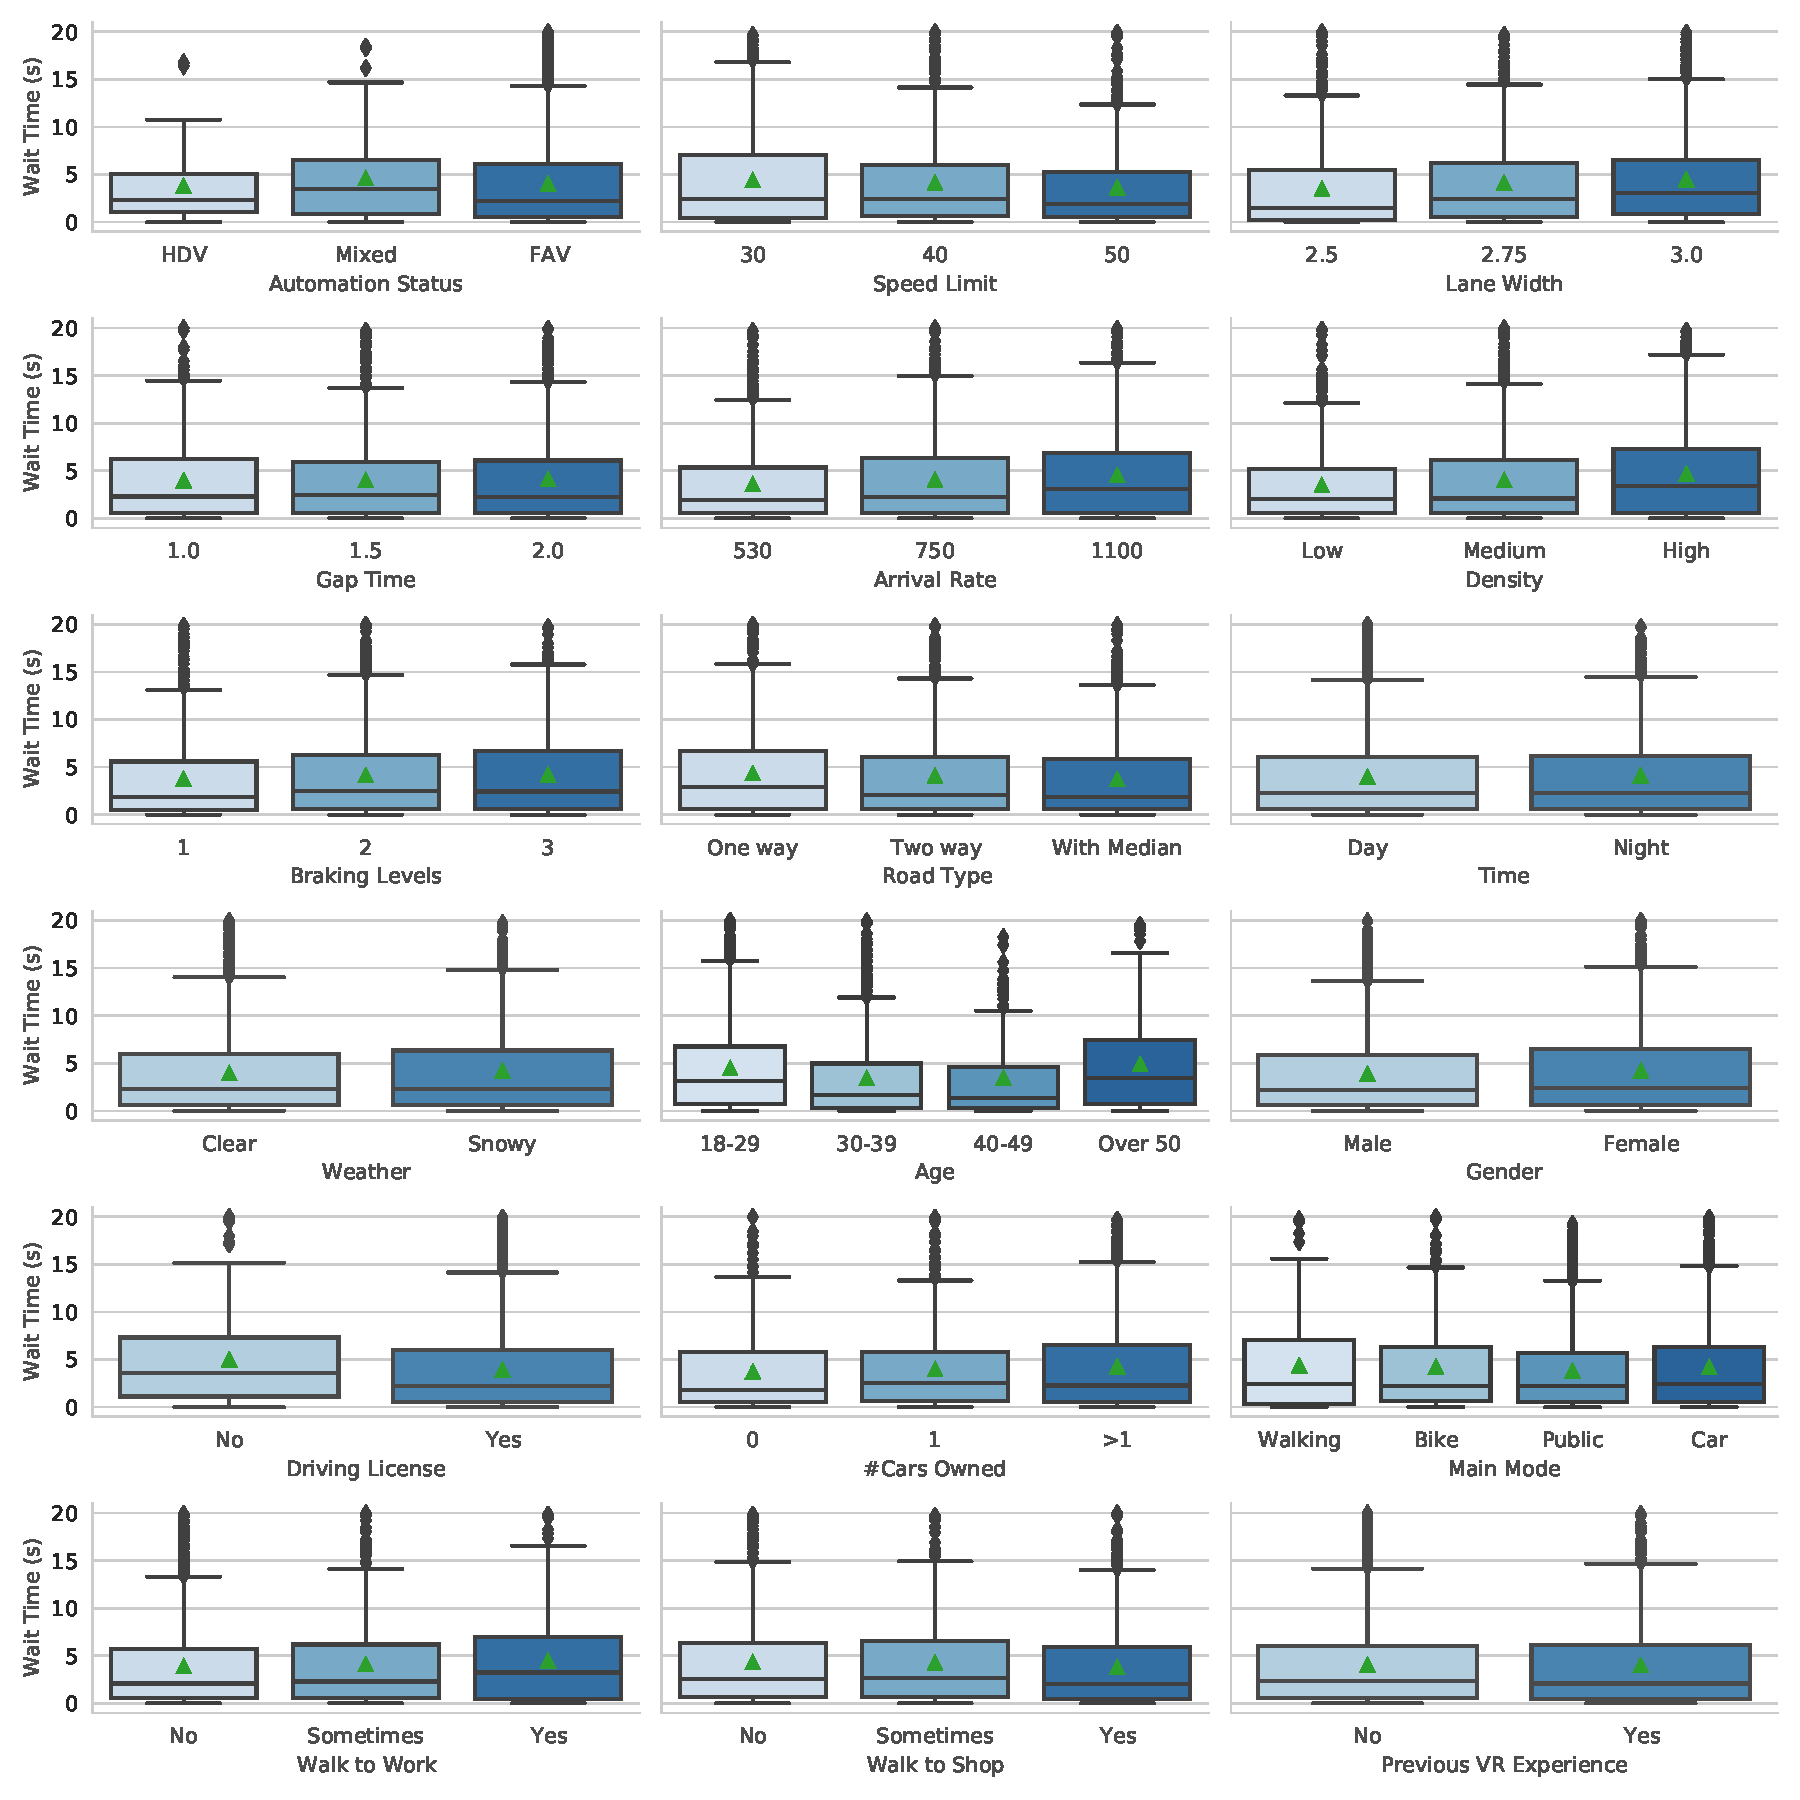
\includegraphics
    [trim=10 10 10 10,clip,width=0.99\textwidth]{chapter_4/figures/comparison.pdf}
    \caption{Comparison of wait time for different levels of covariates}
    \label{fig:comparison}
\end{figure}
\newpage